\section{Evaluation datasets} \label{section:evaluation-datasets}
The experimentally designed features' relevancy is first proven in comparison to comprehensive benchmark datasets. There are a few standardized datasets used in the related work, e.g. \cite{ribeiro_rotating_2017}.

\emph{MaFaulDa} dataset combines vibration and acoustic measurements of the shaft in deviating positions and bearings abnormalities. \emph{CWRU dataset} focuses solely on faults in ball bearings. Another less known dataset concerns shaft unbalance, but compared to the previous two, it demonstrates behavior during revolution speed up.  

\subsection{Machinery Fault Database}
MaFaulDa\footnote{\url{https://www02.smt.ufrj.br/~offshore/mfs/page_01.html}} is a collection of 1951 multivariate time series for 4 different operational conditions on rotor kit Alignment Balance Vibration Trainer (ABVT)~(Fig.~\ref{fig:mafaulda-simulator}). Each series has 5~seconds in duration and is captured at 50 kHz. Vibration signals were obtained with piezoelectric accelerometers with a linear response up to 10~kHz, amplitude range to $\pm$490 $m/s^2$, and resolution step of 10.2~mV per $m/s^2$. 

\begin{figure}[h]
\centering
\begin{subfigure}[b]{0.48\textwidth}
	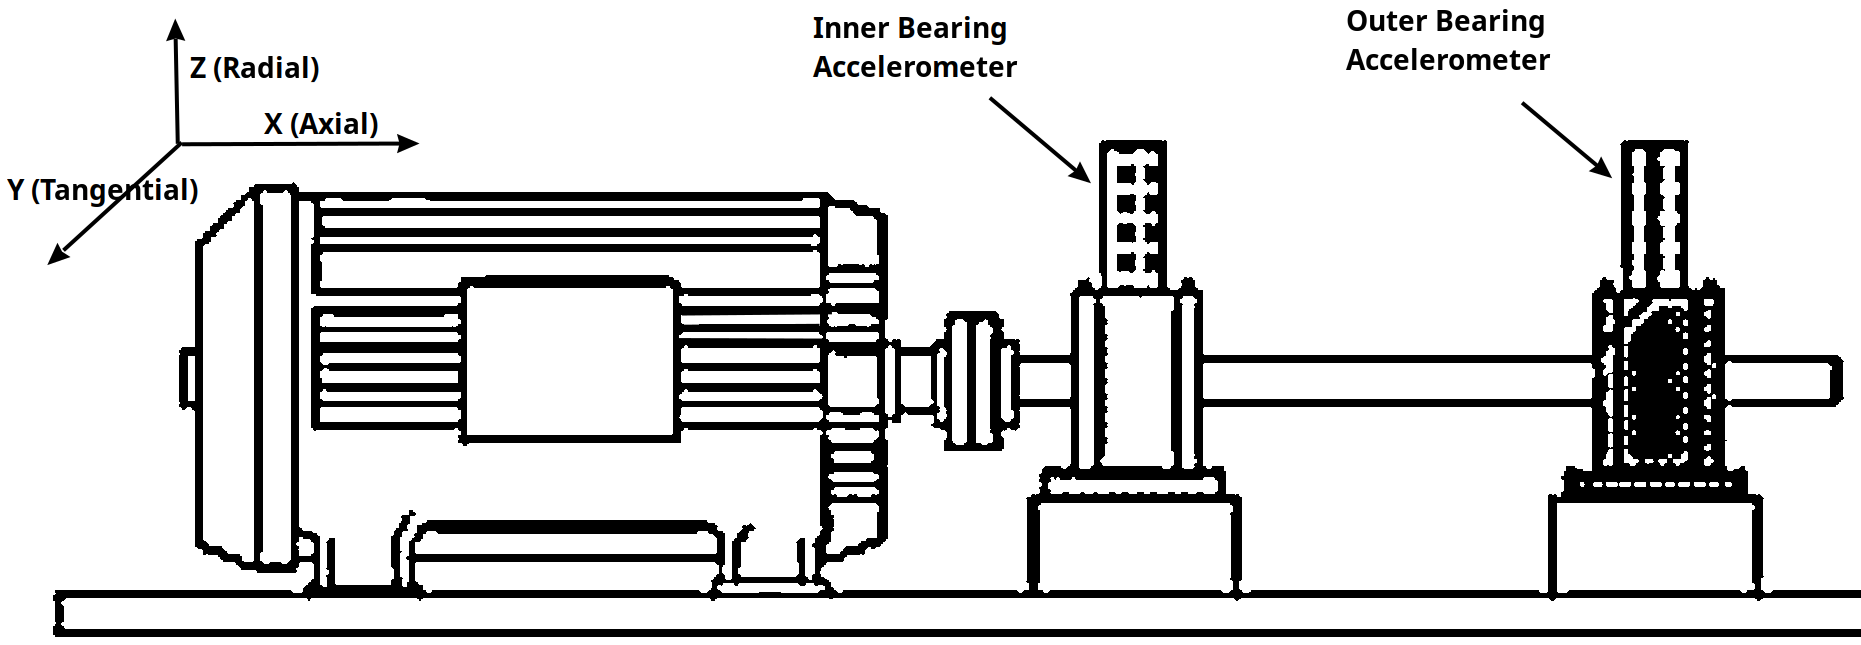
\includegraphics[width=\textwidth]{assets/mafaulda-simulator.png}
	\caption{Schematic diagram \cite{pestana-viana_influence_2016}}
\end{subfigure}
\hfill
\begin{subfigure}[b]{0.48\textwidth}
	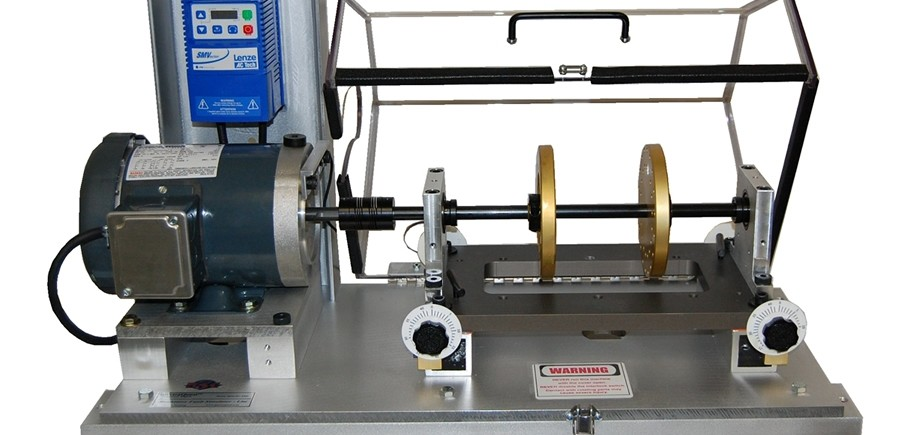
\includegraphics[width=\textwidth]{assets/machinery-fault-simulator.jpg}
	\caption{Mechanical construction \cite{noauthor_spectraquest_nodate}}
\end{subfigure}
\caption{Machinery fault simulator for MaFaulDa}
\label{fig:mafaulda-simulator}
\end{figure}

Observations were conducted in three cardinal axes simultaneously with 2 sets of accelerometers each one associated with one bearing (inner and outer bearings)~(Fig.~\ref{fig:mafaulda-simulator}). Additionally, a magnetic tachometer produced a pulse on shaft turn. The cardioid condenser microphone recorded sound emissions with a frequency range 20~Hz - 20~kHz. Sensors were fed into a four-channel dynamic signal acquisition module. 

Columns in the dataset are organized as depicted in table~\ref{tab:mafaulda-columns}. Machine rotational speeds were kept constant during a particular measurement, but covered a range from 737 to 3686~rpm with steps of approximately 60 rpm (equiv. 10~Hz - 60~Hz)~\cite{pestana-viana_influence_2016}. The maximal rotational frequency achieved with a high unbalance load is 3300 rpm.

\begin{table}[h]
\renewcommand{\arraystretch}{1.2}
\centering
\begin{tabular}{|l|l|}
\hline
\textbf{Columns} & \textbf{Description}                                                                                                                                               \\ \hline
1.               & \begin{tabular}[c]{@{}l@{}}Pulse with modulation of tachometer signal \\ to estimate rotation frequency  (in TTL levels)\end{tabular}                              \\ \hline
2., 3., 4.       & \begin{tabular}[c]{@{}l@{}}Underhang bearing accelerometer \\ (inner - between the rotor and motor)\\ - axial, radial, tangential direction\end{tabular}           \\ \hline
5., 6., 7.       & \begin{tabular}[c]{@{}l@{}}Overhang  bearing accelerometer \\ (Outer - outside most position after the rotor)\\ - axial, radial, tangential direction\end{tabular} \\ \hline
8.               & Microphone                                                                                                                                                         \\ \hline
\end{tabular}
\caption{MaFaulDa description of columns}
\label{tab:mafaulda-columns}
\end{table}

This database contains normal operating conditions, faults out of unbalance, horizontal and vertical shaft misalignment, and three types of faulty bearings in inner and outer positions: outer track, inner track, rolling elements~\cite{pestana-viana_influence_2016}.
\begin{itemize}
\itemsep0pt
\item \textbf{Normal} conditions are baseline without the adverse effect of fault in 49 different rotation speeds. 
\item \textbf{Unbalance} shaft time series uses 8 unbalancing weights from 6 to 35 grams and varying 45 - 49 speeds for each weight adding to 333 mass unbalance loads. 
\item \textbf{Vertical misalignment} set is comprised of 50 signals each (or 51 in one instance) obtained under displacements: 0.51, 0.63, 1.40, 1.90, 1.27, 1.78 mm.
\item \textbf{Horizontal misalignment} signals were recorded under displacements: 0.50, 1.00, 1.50, 2.00 mm, each with 49 different speeds (or 50 in one instance)~\cite{pestana-viana_influence_2016}.
\item \textbf{Bearing faults} are unnoticeable without unbalance. Therefore, weights of 6, 20, and 35 grams were attached to induce a detectable effect. Each unbalance mass was combined with cage, outer race, and ball faults at multiple rotation speeds, usually at 50 different speeds.
\end{itemize}


\subsection{CWRU bearings dataset}
In Case Western Reserve University (CWRU) bearing dataset\footnote{\url{https://engineering.case.edu/bearingdatacenter/download-data-file}} recordings were made of a fan end and drive end bearings under motor loads of 0, 1, 2, and 3~Horsepower (equivalently 0, 0.75, 1.49, 2.24~kW). Shaft speed was unaltered in all experiments, but it fluctuated between 1720 and 1797~rpm (approx. 29~Hz).

\begin{figure}[h]
\begin{subfigure}[b]{0.48\textwidth}
	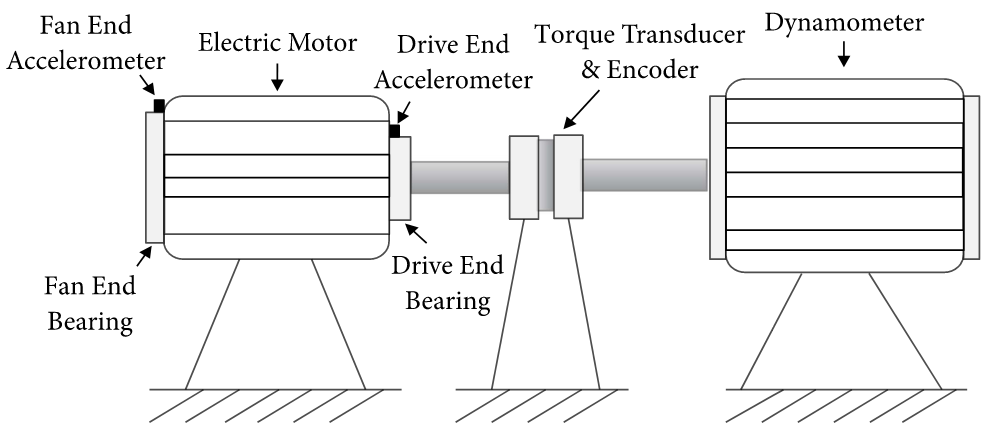
\includegraphics[width=\textwidth]{assets/cwru-test-stand-2.png}
	\caption{Schematic diagram \cite{song_bearing_2022}}
\end{subfigure}
\hfill
\begin{subfigure}[b]{0.48\textwidth}
	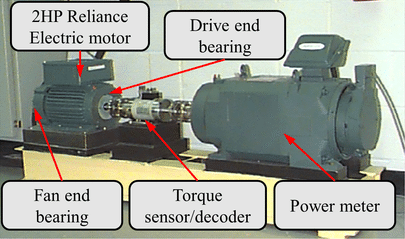
\includegraphics[width=\textwidth]{assets/cwru-test-stand.png}
	\caption{Mechanical construction \cite{yuhong_new_2021}}
\end{subfigure}
\caption{CWRU machine apparatus}
\label{fig:cwru-simulator}
\end{figure}

Single point defects were created with diameters of 0.007, 0.014, 0.021, 0.028, and 0.040 inches (equivalently 0.18, 0.36, 0.72, 1.02 mm). Fault locations on bearings are in the inner raceway, in the outer raceway directly and orthogonally relative to the load zone, and on rolling ball elements~(Fig.~\ref{fig:cwru-simulator})~\cite{jamil_feature-based_2021}. 

\begin{table}[h]
\centering
\renewcommand{\arraystretch}{1.2}
\begin{tabular}{|l|l|}
\hline
\textbf{Columns} & \textbf{Description}                 \\ \hline
1. DE        & Drive end accelerometer samples 		\\ \hline
2. FE        & Fan end accelerometer samples   			\\ \hline
3. BA        & Base accelerometer samples (optional)   \\ \hline
4. RPM     & Rotation speed of the motor in rpm        \\ \hline
\end{tabular}
\caption{CWRU dataset description of columns}
\label{tab:cwru-columns}
\end{table}

The sampling frequency during baseline set, drive end, and fan end bearing capture is 12 kHz, exclusively for drive end bearings samples were taken at 48 kHz. The duration of the time series is varied from 5 to 40 seconds. Drive end and fan end bearings signals are measured in each experiment. Accelerometer was sometimes mounted on the supporting base plate.

\subsection{Unbalance of the rotating shaft}
Unbalance Detection of a Rotating Shaft\footnote{\url{https://www.kaggle.com/datasets/jishnukoliyadan/vibration-analysis-on-rotating-shaft}} is a Kaggle dataset that simulates 4 different unbalance strengths. 
\begin{figure}[h]
\centering
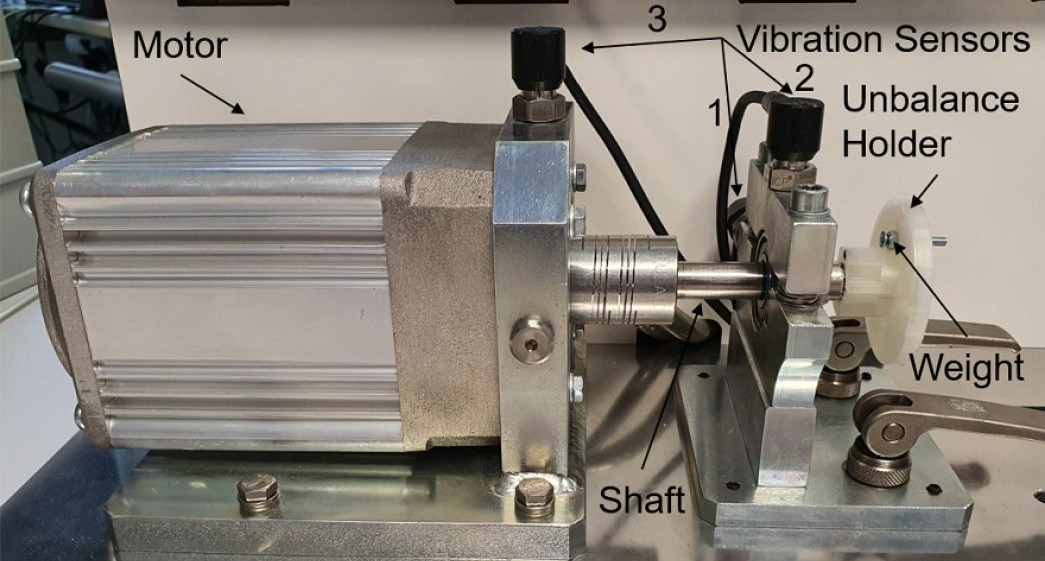
\includegraphics[width=0.7\textwidth]{assets/rotating-shaft.jpg}
\caption{Motor driving shaft in unbalance measurement \cite{mey_machine_2020}}
\label{fig:rotating-shaft}
\end{figure}

The setup is shown in Fig.~\ref{fig:rotating-shaft}. Mass of 3.28 grams (or 6.61 grams during severe unbalance test) is attached to unbalance holder successively in 5 sets (numbered 0 - 4) on the radii 0, 14, 18.5, 23, 23 mm. The rotation speed of the motor is perpetually rising between 630 and 2330 rpm in development datasets (marked with suffix D) and speeds from 1060 to 1900 rpm in the evaluation datasets (suffix E). The vibrations were recorded at a sampling rate of 4 kHz~\cite{mey_machine_2020}.

\begin{table}[h]
\centering
\renewcommand{\arraystretch}{1.2}
\begin{tabular}{|l|l|}
\hline
\textbf{Columns} & \textbf{Description}                      \\ \hline
1. V\_in         & Input voltage to the motor controller (V) \\ \hline
2. Measured\_RPM & Rotation speed of the motor (rpm)  \\ \hline
3. Vibration\_1  & 1. Vibration sensor (samples)             \\ \hline
4. Vibration\_2  & 2. Vibration sensor (samples)             \\ \hline
5. Vibration\_3  & 3. Vibration sensor (samples)             \\ \hline
\end{tabular}
\caption{``Unbalance on the rotating shaft'' dataset description of columns}
\end{table}

The accelerometers used are piezoelectric and have a frequency range of up to 10 KHz, dynamic range of $\pm$490 $m/s^2$, and resolution step of 10.2~mV per $m/s^2$. These sensor parameters are the same as in the case of MaFaulDa. In total, three different uniaxial accelerometers are mounted on the motor housing.
